\documentclass[12pt, a4paper]{article}
\usepackage[utf8]{inputenc}
\usepackage[brazilian]{babel}
\usepackage[T1]{fontenc}
\usepackage{lipsum}
\usepackage{graphicx}
	\graphicspath{{images/}}

\title{Olá, Mundo!}
\author{Willem Romão}
\date{\today}

\begin{document}
	\maketitle
	\begin{abstract}
		\lipsum[1]
	\end{abstract}
	
	\section{Quid est veritas?}
		\lipsum[2]
		
		\subsection{Est vir qui adest}
			\lipsum[3-4]
			
			\begin{figure}[!htpb]
				\centering
				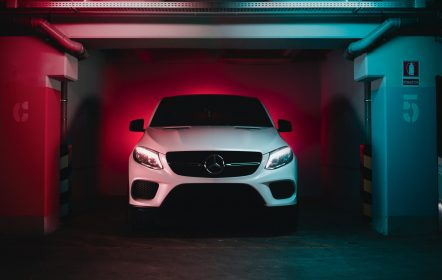
\includegraphics[width=0.5\textheight]{car-garage.jpg}
				\caption{Diagrama de espaço--tempo para o paradoxo do carro e da, 
					garagem.}
				\label{fig: car-garage}
				
			\end{figure}
		
		Figura \ref{fig: car-garage} na página \pageref{fig: car-garage}
		
		\begin{table}[!htbp]
			\centering
			\caption{Exemplos de números representados em base binária}
			\label{tab: binary}
			\begin{tabular}{c|c}
				 Base Decimal & Base Binária \\ \hline
				 1 & 1 \\
				 2 & 10 \\
				 3 & 11 \\
				 4 & 100 \\
				 5 & 101 
				 
			\end{tabular}	
		\end{table}
			
\end{document}
